\section{Additional Known-Dependence Resource Evidence}
\subsection{Correlation-limited participation}
The participation study varies $q\in\{1,2,4,8,16,32\}$, six cross-agent correlation levels, three delays, three message-equivalent budgets, and thirteen step sizes over 32 paired seeds.
At $q=32$, median effective participation is $30.996$ for independent trajectories and $1.111$ at correlation $0.9$.
At the largest evaluated budget and delay eight, the resource-optimal participation moves from $q=16$ under independence to $q=1$ under high sharing.
Using the endpoint action selected for the opposite correlation regime increases error by factors of approximately $4.29$ and $3.13$, respectively.
Equal charged endpoint budgets isolate the value of dependence-matched participation.

\subsection{Finite-time certificate and joint actions}
The joint-action study evaluates twelve $(\text{persistence},\rho,D)$ scenarios with 32 new paired seeds and 1,152 policy runs.
The joint controller searches a stability-screened catalogue of $q\in\{1,2,4,8,16,32\}$, charged spacings, and scalar steps.
All selected actions satisfy $0<c_{\rm aff}<1$ and the declared budget.
The finite-time bound beats the no-update risk in all twelve scenarios (12/12).
Every one-sided 99 percent bootstrap upper mean lies below its corresponding bound, with a maximum empirical-upper-bound to theorem-bound ratio of $0.305$.
The median theorem-bound to empirical-mean ratio is $20.77$ and the maximum is $228.98$.
The selected actions show how the certificate responds to correlation, delay, and persistence despite this slack.
Mean participation is $12.67$ for independent sources and $q=1$ in every high-sharing scenario.
Delay reduces the selected independent-source participation to $q=4$, while raising temporal persistence from zero to $0.98$ increases the median paid spacing by a factor of $18.49$.
Fig.~\ref{fig:joint-actions} retains the complete action plot.

\subsection{Held-out resource-indexed convergence curves}
Fig.~\ref{fig:convergence-curves} shows the persistence-$0.9$, zero-delay slice: broad participation accelerates independent-source learning, whereas low participation avoids the shared-noise floor.
\begin{figure*}[t]
\centering
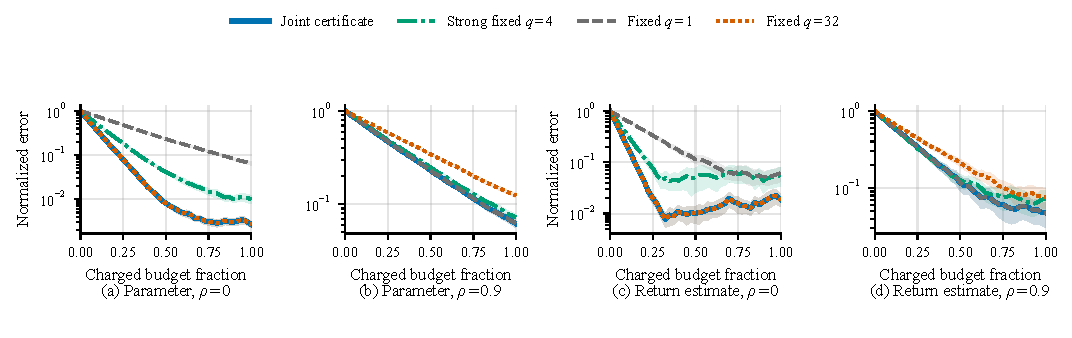
\includegraphics[width=0.96\textwidth]{figures/convergence_curves.pdf}
\caption{Held-out resource-indexed convergence for persistence $0.9$ and zero delay (64 confirmation seeds; bands are 95 percent confidence intervals).
The first two panels show parameter risk and the last two return-estimation risk, compared with the development-selected fixed $q=4$.}
\label{fig:convergence-curves}
\end{figure*}
